\chapter{Introduction}
\setcounter{page}{1}


Lorem ipsum dolor sit amet, consectetur adipiscing elit. Aenean malesuada, tellus eget dignissim cursus, odio libero varius ex, quis finibus libero odio eget nulla. In eu mauris finibus leo faucibus lobortis at et nunc. Nulla gravida vitae nulla at porttitor. Proin nisl nulla, efficitur in auctor ut, semper ut orci. Donec sit amet sapien mollis, placerat ex id, tempor purus. Praesent ac cursus quam. Pellentesque habitant morbi tristique senectus et netus et malesuada fames ac turpis egestas. Nunc purus est, dignissim in elit ac, auctor congue mi. Pellentesque blandit lorem eu fermentum sagittis. Nulla feugiat, magna non placerat laoreet, tellus dui laoreet nisl, id feugiat sapien enim sit amet felis. Etiam mattis, felis in fermentum accumsan, justo odio mollis diam, ut faucibus nulla nisl sit amet leo. Donec fringilla bibendum augue eget vestibulum.

Suspendisse eget euismod lectus, at cursus ex. Donec volutpat nunc vitae justo hendrerit porttitor. Aenean ut sem lobortis, convallis sapien at, tincidunt arcu. Praesent ornare sem est, eu pulvinar elit volutpat quis. Nam sollicitudin, arcu id mollis aliquam, dolor quam posuere dui, eu hendrerit erat urna egestas nisl. In posuere ante et dolor pretium mollis. Integer bibendum metus in lacus ornare rutrum. As shown in \ref{bigData}



\begin{figure}[h]
    \centering
    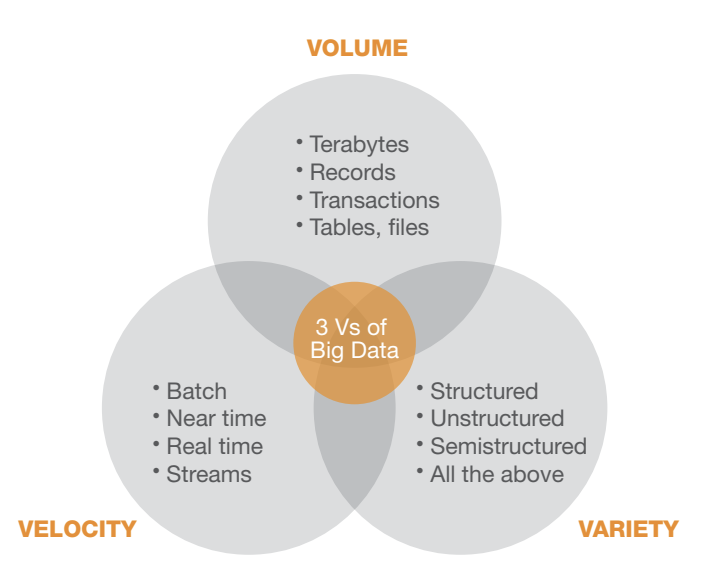
\includegraphics[width=0.5\textwidth]{images/big_data.png}
    \caption{Big Data: 3 V's}
    \label{bigData}
\end{figure}

\section{Section 1}

This is a test reference to \autocite{king_anthony_2022}.


Maecenas imperdiet neque vestibulum lorem convallis tristique. Sed orci ex, ornare in cursus eu, placerat quis ligula. In ornare ornare pretium. Ut a ipsum quis sem gravida lacinia a eu elit. Nulla pellentesque tincidunt tempus. Mauris dui neque, tincidunt sed consectetur nec, volutpat ut dolor. Etiam eget pellentesque lectus. Phasellus at ipsum imperdiet, cursus tellus non, maximus massa. Ut ut laoreet neque. Morbi vestibulum, lectus ac tristique tincidunt, ex sem dictum diam, accumsan tempor velit velit non risus. Nunc pharetra, neque non accumsan ornare, purus mi dignissim turpis, a pellentesque quam purus in purus. Aliquam erat volutpat. Cras viverra nibh vel enim blandit semper. Phasellus tincidunt pellentesque aliquam. Sed sed nisl eget eros interdum malesuada. In eget facilisis tellus, condimentum condimentum tortor.

Maecenas quis nisi vitae nulla sollicitudin blandit ac ac eros. Ut id imperdiet nulla. Morbi rutrum arcu bibendum dictum fermentum. Nulla ut pharetra tellus, quis hendrerit eros. Phasellus eros leo, faucibus ut mattis eu, malesuada eu metus. Curabitur faucibus metus nec nunc porta ultrices. Praesent ullamcorper purus ac mauris sollicitudin facilisis. Mauris vel elit mollis, ornare neque vitae, fringilla felis. Morbi a sapien vel velit ultricies fringilla.

Vestibulum malesuada tempor hendrerit. Suspendisse libero libero, venenatis in nisi et, mattis egestas arcu. Sed vitae lobortis magna. Aenean placerat vitae massa at mollis. Nam laoreet mollis diam sed commodo. Proin dapibus erat sem, ac molestie diam volutpat at. Mauris venenatis dolor in ante cursus, in consectetur leo pretium. Duis metus mi, porttitor vel eros quis, blandit interdum ligula. Nam lorem lacus, ultricies id laoreet a, luctus consequat odio. Sed ut orci et leo vulputate viverra non vel eros. Etiam vel magna in ex dapibus pretium. Integer rutrum nunc vitae molestie dictum. Donec vehicula sem et justo efficitur fringilla. Vestibulum pellentesque lorem eget lacinia finibus. Praesent accumsan elit id magna efficitur imperdiet. Sed nibh massa, molestie quis dapibus eu, finibus eget libero.

As the name suggests, big data is a large amount of data. There are other important attributes of big data. These are:  data variety and data velocity.

Thus we can define big data using 3 V's: \textit{volume}, \textit{variety}, and \textit{velocity} as showin in Figure \ref*{bigData}.
\section{Section 2}

This is a test reference to \autocite{king_anthony_2022}.


Maecenas imperdiet neque vestibulum lorem convallis tristique. Sed orci ex, ornare in cursus eu, placerat quis ligula. In ornare ornare pretium. Ut a ipsum quis sem gravida lacinia a eu elit. Nulla pellentesque tincidunt tempus. Mauris dui neque, tincidunt sed consectetur nec, volutpat ut dolor. Etiam eget pellentesque lectus. Phasellus at ipsum imperdiet, cursus tellus non, maximus massa. Ut ut laoreet neque. Morbi vestibulum, lectus ac tristique tincidunt, ex sem dictum diam, accumsan tempor velit velit non risus. Nunc pharetra, neque non accumsan ornare, purus mi dignissim turpis, a pellentesque quam purus in purus. Aliquam erat volutpat. Cras viverra nibh vel enim blandit semper. Phasellus tincidunt pellentesque aliquam. Sed sed nisl eget eros interdum malesuada. In eget facilisis tellus, condimentum condimentum tortor.

Maecenas quis nisi vitae nulla sollicitudin blandit ac ac eros. Ut id imperdiet nulla. Morbi rutrum arcu bibendum dictum fermentum. Nulla ut pharetra tellus, quis hendrerit eros. Phasellus eros leo, faucibus ut mattis eu, malesuada eu metus. Curabitur faucibus metus nec nunc porta ultrices. Praesent ullamcorper purus ac mauris sollicitudin facilisis. Mauris vel elit mollis, ornare neque vitae, fringilla felis. Morbi a sapien vel velit ultricies fringilla.

Vestibulum malesuada tempor hendrerit. Suspendisse libero libero, venenatis in nisi et, mattis egestas arcu. Sed vitae lobortis magna. Aenean placerat vitae massa at mollis. Nam laoreet mollis diam sed commodo. Proin dapibus erat sem, ac molestie diam volutpat at. Mauris venenatis dolor in ante cursus, in consectetur leo pretium. Duis metus mi, porttitor vel eros quis, blandit interdum ligula. Nam lorem lacus, ultricies id laoreet a, luctus consequat odio. Sed ut orci et leo vulputate viverra non vel eros. Etiam vel magna in ex dapibus pretium. Integer rutrum nunc vitae molestie dictum. Donec vehicula sem et justo efficitur fringilla. Vestibulum pellentesque lorem eget lacinia finibus. Praesent accumsan elit id magna efficitur imperdiet. Sed nibh massa, molestie quis dapibus eu, finibus eget libero.

\subsection{Subsection 1}

There is a table in this section which can be refered using label \ref{tab:mytable}.

\begin{table}[h]
    \centering
    \begin{tabular}{|c|c|c|}
        \hline
        Column 1        & Column 2        & Column 3        \\
        \hline
        Row 1, Column 1 & Row 1, Column 2 & Row 1, Column 3 \\
        Row 2, Column 1 & Row 2, Column 2 & Row 2, Column 3 \\
        \hline
    \end{tabular}
    \caption{This is a table with three columns and two rows.}
    \label{tab:mytable}
\end{table}

we can also add charts. More chart types coming soon.


\begin{tikzpicture}
    \draw[->] (0,0) -- (6,0) node[right] {$x$};
    \draw[->] (0,0) -- (0,4) node[above] {$y$};
    \draw[domain=0:2,smooth,variable=\x,blue] plot ({\x},{0.5*\x^2});
    \node at (3,2) {$y=\frac{1}{2}x^2$};
\end{tikzpicture}

